% On découpe ce document complexe en plusieurs sous-fichiers séparés.
% Cela permettra notamment de réarranger les transparents facilement 
% lors de l'élaboration du document.

% La définition de la classe beamer avec tous les styles afférents

\documentclass[9pt]{beamer}

\input{preambule/special_beamer.tex}

% Les autres packages utiles  notamment pour le français, les accents ou Python
\usepackage{url}            % Pour citer les adresses web
\usepackage[T1]{fontenc}    % Encodage des accents
\usepackage[utf8]{inputenc} % Lui aussi
\usepackage[french]{babel}  % Pour la traduction française
\usepackage{numprint}       % Histoire que les chiffres soient bien

\usepackage{amsmath}        % La base pour les maths
\usepackage{mathrsfs}       % Quelques symboles supplémentaires
\usepackage{amssymb}        % encore des symboles.
\usepackage{amsfonts}       % Des fontes, eg pour \mathbb.

\usepackage{cancel}

\usepackage{caption}
\captionsetup[figure]{
  labelformat=simple,       % affiche juste le numéro
  labelsep=period,          % séparateur point
  name=Fig.,                % remplace "Figure" par "Fig."
  font=scriptsize,          % texte très petit (ou "tiny" encore plus petit)
  skip=2pt                  % espace minimal entre figure et caption
}

\usepackage[backend=biber, style=numeric, sorting=none]{biblatex}
\addbibresource{references.bib}

%\usepackage[svgnames]{xcolor} % De la couleur

%%% Si jamais vous voulez changer de police: décommentez les trois 
%\usepackage{tgpagella}
%\usepackage{tgadventor}
%\usepackage{inconsolata}


\usepackage{graphicx} % inclusion des graphiques
\usepackage{wrapfig}  % Dessins dans le texte.

\usepackage{tikz}     % Un package pour les dessins (utilisé pour l'environnement {code})
\usetikzlibrary{calc, patterns, arrows.meta, positioning}
\usepackage[framemethod=TikZ]{mdframed}
\usepackage{tcolorbox}

% Les macros et raccourcis personnels
% Ce fichier contient toutes les macros que vous pouvez avoir envie de définir 
% si vous les utilisez plusieurs fois dans le document.

\PassOptionsToPackage{svgnames}{color}

% Un environnement pour bien présenter le code informatique
\newenvironment{code}{%
\begin{mdframed}[linecolor=green,innerrightmargin=30pt,innerleftmargin=30pt,
backgroundcolor=black!5,
skipabove=10pt,skipbelow=10pt,roundcorner=5pt,
splitbottomskip=6pt,splittopskip=12pt]
}{%
\end{mdframed}
}


% On définit le titre et l'auteur du document

% L'argument optionnel (entre crochets) donne le titre qui sera mis sur chaque slide
\title[TIPE Pendule Inversé]{Stabilisation active de systèmes en équilibre instable:\newline du pendule aux lanceurs réutilisables}
\author{Thibaut \textsc{Dehaeze (26351)}} % Votre nom
% L'épreuve (car on n'a pas le droit de signaler sa provenance à un concours) (là encore, l'argument optionnel apparaît sur chaque slide)
\institute[TIPE]{Épreuve de TIPE}
\date{Session 2026}

% On démarre le document proprement dit
\begin{document}

\begin{frame}
\titlepage 
\end{frame}

% La première grande partie: introduction du sujet
\section{Introduction}

\begin{frame}
\frametitle{Introduction}
\framesubtitle{Applications}

\begin{figure}
    \begin{minipage}[t]{0.32\linewidth}
        \centering
        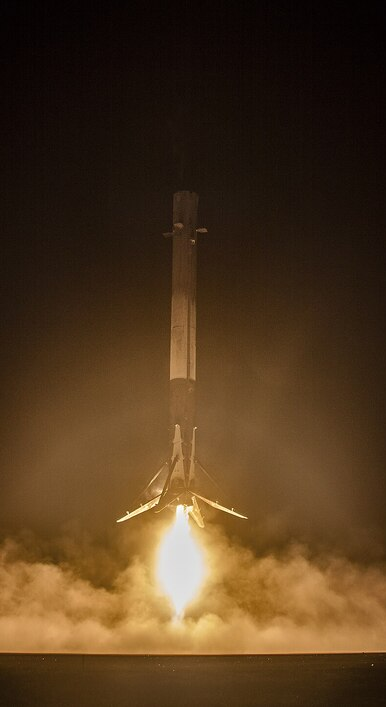
\includegraphics[height=4.5cm]{figures/lanceur_reutilisable.jpg}\\[2pt]
        \parbox{\linewidth}{\centering\scriptsize Lanceur Réutilisable~\cite{spacex}}
    \end{minipage}\hfill
    \begin{minipage}[t]{0.32\linewidth}
        \centering
        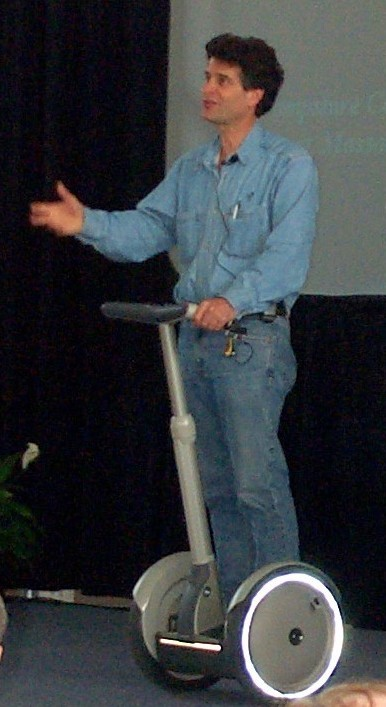
\includegraphics[height=4.5cm]{figures/segway.jpg}\\[2pt]
        \parbox{\linewidth}{\centering\scriptsize Segway~\cite{segway}}
    \end{minipage}\hfill
    \begin{minipage}[t]{0.32\linewidth}
        \centering
        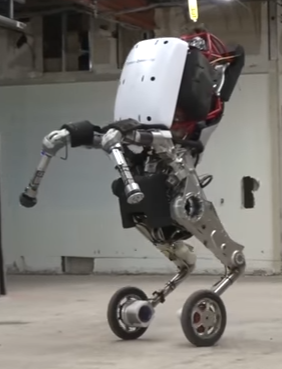
\includegraphics[height=4.5cm]{figures/self_balancing_robot.png}\\[2pt]
        \parbox{\linewidth}{\centering\scriptsize Robot auto-équilibré~\cite{bostondynamics}}
    \end{minipage}
\end{figure}

\end{frame}

%%%%%%%%%%%%%%%%%%%%%%%%%%%%%%%%%%%%%%%%%%%%%%%%

\begin{frame}
\frametitle{Introduction}
\framesubtitle{Le Pendule Inversé}

\begin{figure}
    \begin{minipage}[t]{0.32\linewidth}
        \centering
        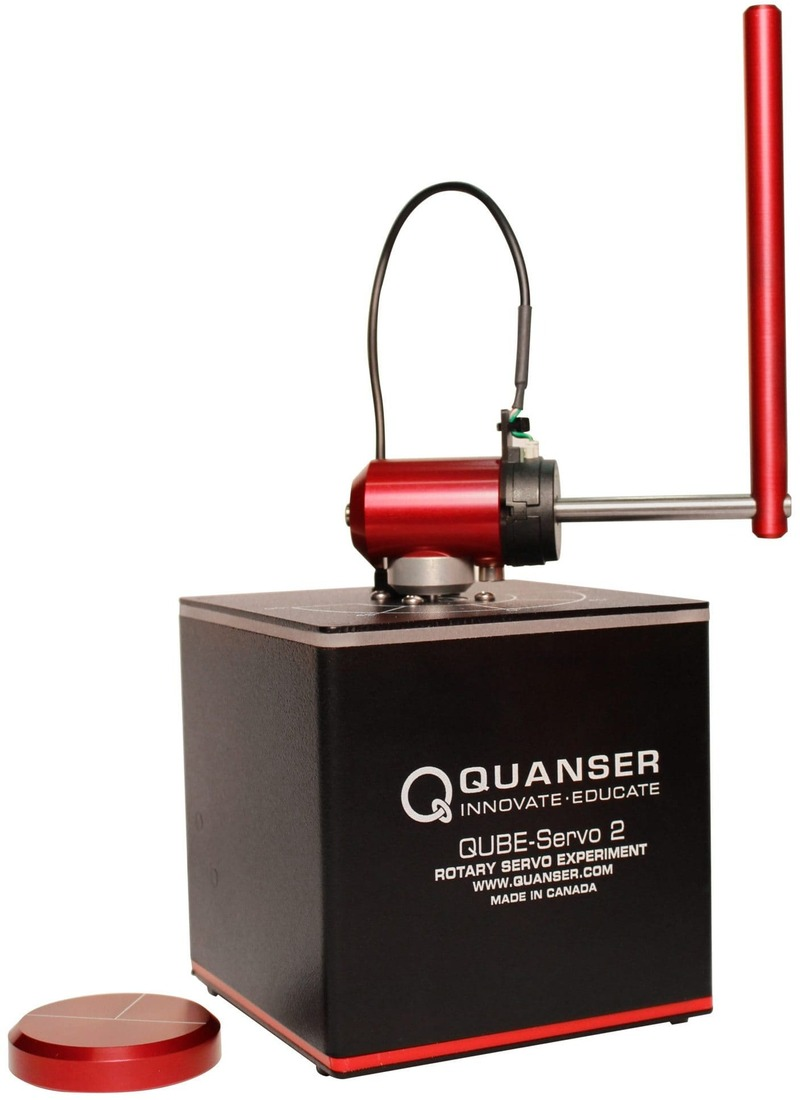
\includegraphics[height=5cm]{figures/inverted_pendulum_rotary.jpg}\\[2pt]
        \parbox{\linewidth}{\centering\scriptsize Pendule inversé rotatif~\cite{quanser_rotary}}
    \end{minipage}\hfill
    \begin{minipage}[t]{0.64\linewidth}
        \centering
        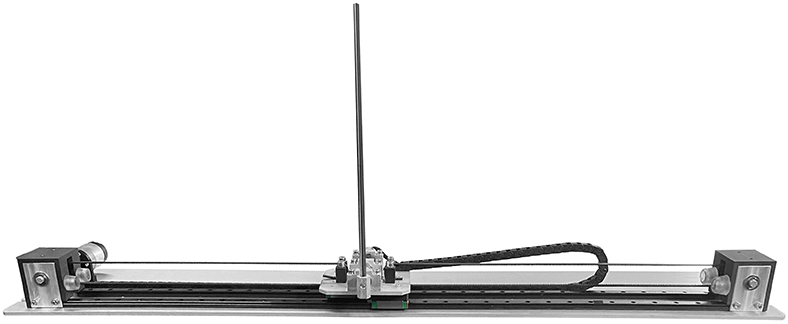
\includegraphics[height=3cm]{figures/inverted_pendulum_linear.png}\\[2pt]
        \parbox{\linewidth}{\centering\scriptsize Pendule inversé sur chariot~\cite{acrome_linear}}
    \end{minipage}
\end{figure}

\end{frame}

%%%%%%%%%%%%%%%%%%%%%%%%%%%%%%%%%%%%%%%%%%%%%%%%

\begin{frame}
\frametitle{Introduction}
\framesubtitle{Problématique}

\vfill
\begin{center}
\begin{tcolorbox}[
    width=0.9\linewidth,
    colback=blue!5,
    colframe=blue!50!black,
    arc=4pt,
    boxrule=1pt,
    fontupper=\large
]
Comment la dynamique d'un système mécanique au voisinage d'un équilibre instable peut-elle être modifiée afin d'assurer sa stabilité au cours du temps, comme dans le cas des lanceurs réutilisables lors de leur retour vertical~?
\end{tcolorbox}
\end{center}
\vfill

\end{frame}

%%%%%%%%%%%%%%%%%%%%%%%%%%%%%%%%%%%%%%%%%%%%%%%%

\begin{frame}
\frametitle{Plan de l'exposé} 
\framesubtitle{Démarche}

\tableofcontents 

\end{frame}


% La 2e partie: Etude de la dynamique
\section{Étude de la dynamique du Pendule Inversé}

\begin{frame}
\frametitle{Étude de la dynamique}
\framesubtitle{Présentation du système}

\begin{figure}
    \only<1>{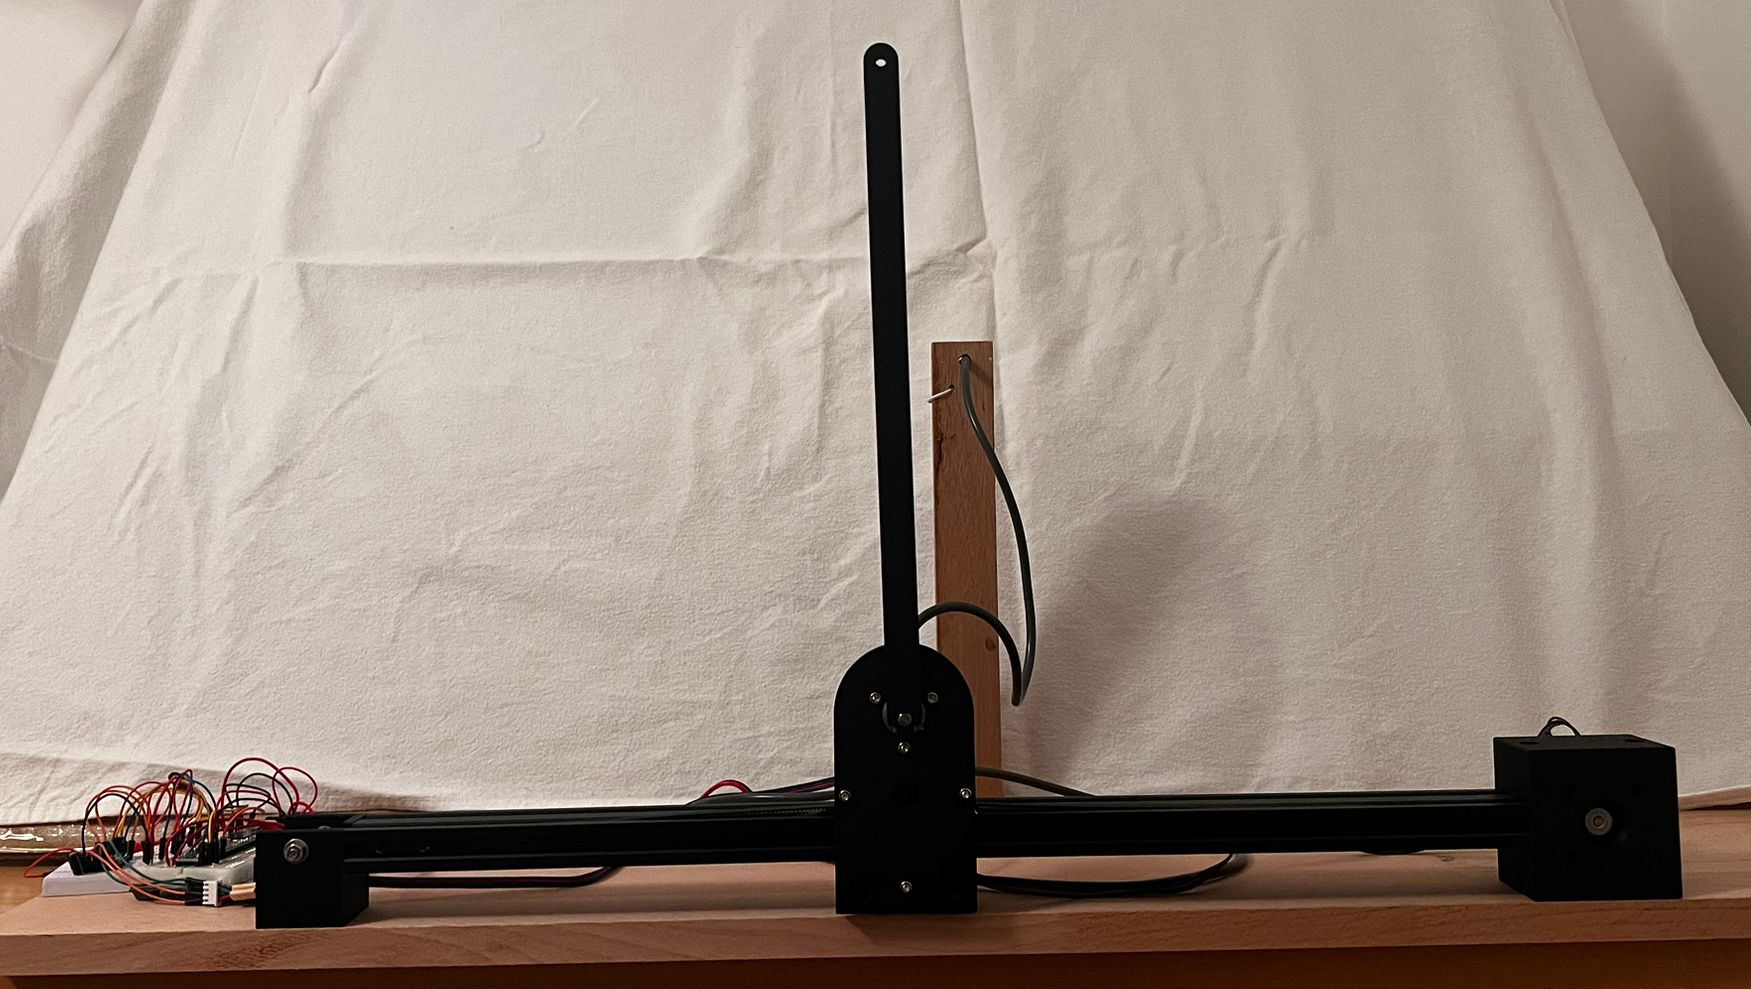
\includegraphics[width=\textwidth]{figures/pendulum-picture.jpg}}%
    \only<2>{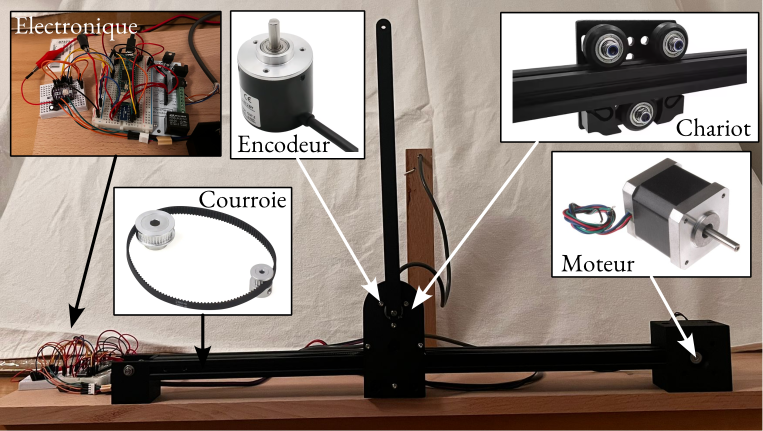
\includegraphics[width=\textwidth]{figures/inverted_pendulum_picture_schematic.png}}
\end{figure}

\end{frame}

%%%%%%%%%%%%%%%%%%%%%%%%%%%%%%%%%%%%%%%%%%%%%%%%

\begin{frame}
\frametitle{Étude de la dynamique}
\framesubtitle{Modèle et Équations de la dynamique}

\begin{columns}[T]

%--- Colonne gauche : schéma ---
\begin{column}{0.45\textwidth}
\begin{center}
\begin{tikzpicture}[>=Stealth, scale=0.8]

  % Ground
  \fill[pattern=north east lines, pattern color=gray!60] (-1.5,-0.18) rectangle (1.5,0);
  \draw[thick] (-1.5,0) -- (1.5,0);

  % Wheels
  \draw[thick, fill=white] (-0.45, 0.15) circle [radius=0.15];
  \draw[thick, fill=white] ( 0.45, 0.15) circle [radius=0.15];

  % Cart body
  \draw[thick, fill=gray!20, rounded corners=3pt]
    (-0.8, 0.15) rectangle (0.8, 0.75);

  % Pivot
  \coordinate (O) at (0, 0.75);
  \fill (O) circle [radius=0.1];

  % Pendulum (theta = 150 deg from downward, 30 deg from upright)
  \coordinate (tip) at ($(O) + ({0.5*3.0}, {0.866*3.0})$);

  % Dashed verticals
  \draw[dashed, gray] (O) -- ++(0,  3.5);
  \draw[dashed, gray] (O) -- ++(0, -0.9);

  % Angle arc (CCW from downward to rod, through right side)
    \draw[->] ($(O)+(-90:0.7)$) arc[start angle=-90, end angle=60, radius=0.7] node[near end, right] {$\theta$};

  % Pendulum rod
  \draw[line width=2pt] (O) -- node[midway, right=6pt] {$m,I$} (tip);

  % Length arrow
  \draw[<->, thin]
    ($(O)   + ({-0.866*0.35}, {0.5*0.35})$)
    -- node[left=2pt] {$l$}
    ($(tip) + ({-0.866*0.35}, {0.5*0.35})$);

  % Tip dot
  \fill (tip) circle [radius=0.05];

  % Acceleration arrow
  \draw[->, very thick, blue!70!black]
    (0.85, 0.44) -- ++(1.0, 0) node[right] {$u = \ddot{x}$};

\end{tikzpicture}
\end{center}
\end{column}

%--- Colonne droite : équations ---
\begin{column}{0.52\textwidth}
  \vspace{0.5cm}
  \textbf{Équation du mouvement :}
  \begin{equation*}
    D\,\ddot{\theta} + c\,\dot{\theta} + mgl\sin\theta + ml\cos\theta\cdot u = 0
  \end{equation*}
  avec $D = I + ml^2 = \dfrac{4}{3}ml^2$
\end{column}

\end{columns}

\end{frame}

%%%%%%%%%%%%%%%%%%%%%%%%%%%%%%%%%%%%%%%%%%%%%%%%

\begin{frame}
\frametitle{Étude de la dynamique}
\framesubtitle{Linéarisations et Réponses du système}

\begin{columns}[T]

\begin{column}{0.48\textwidth}
  \centering\textbf{Position basse} ($\theta \approx 0$)
  \begin{equation*}
    D\,\ddot{\theta} + c\,\dot{\theta} + mgl\,\theta = 0
  \end{equation*}
  $\Rightarrow$ Oscillations amorties

  \begin{figure}
      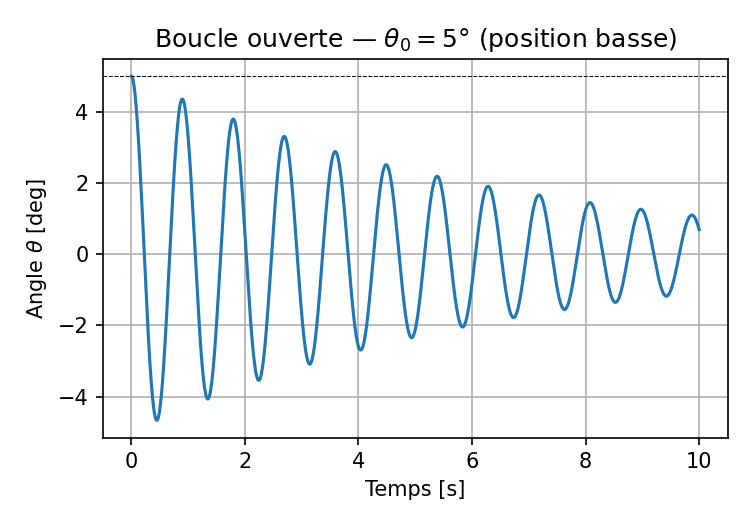
\includegraphics[width=\linewidth]{figures/openloop_5deg.png}
  \end{figure}
\end{column}

\begin{column}{0.48\textwidth}
  \centering\textbf{Position haute} ($\varphi = \theta - \pi \approx 0$)
  \begin{equation*}
    D\,\ddot{\varphi} + c\,\dot{\varphi} - mgl\,\varphi = 0
  \end{equation*}
  $\Rightarrow$ Divergence exponentielle

  \begin{figure}
      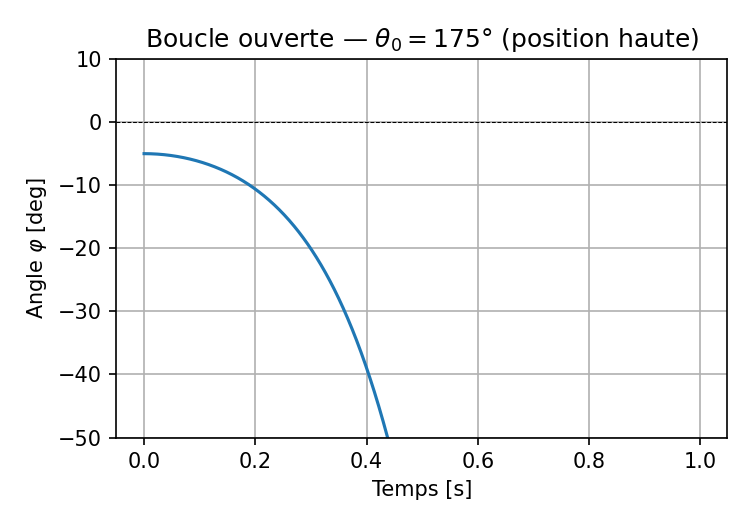
\includegraphics[width=\linewidth]{figures/openloop_175deg.png}
  \end{figure}
\end{column}

\end{columns}

\end{frame}

%%%%%%%%%%%%%%%%%%%%%%%%%%%%%%%%%%%%%%%%%%%%%%%%

\begin{frame}
\frametitle{Étude de la dynamique}
\framesubtitle{Comparaison modèle / expérience}

\begin{center}
\begin{tikzpicture}[>=Stealth,
    box/.style={draw, rounded corners=4pt, fill=blue!8, text width=2.8cm,
                align=center, minimum height=1.2cm, font=\small},
    arr/.style={->, thick, blue!60!black}
  ]

  \node[box] (meas) {Mesure de la\\réponse\\expérimentale};
  \node[box, right=1.2cm of meas] (opt)  {Optimisation\\des paramètres\\du modèle};
  \node[box, right=1.2cm of opt]  (res)  {Paramètres\\identifiés\\$m,\ l,\ c$};

  \draw[arr] (meas) -- (opt);
  \draw[arr] (opt)  -- (res);

\end{tikzpicture}
\end{center}

\vspace{0.2cm}

\begin{figure}
    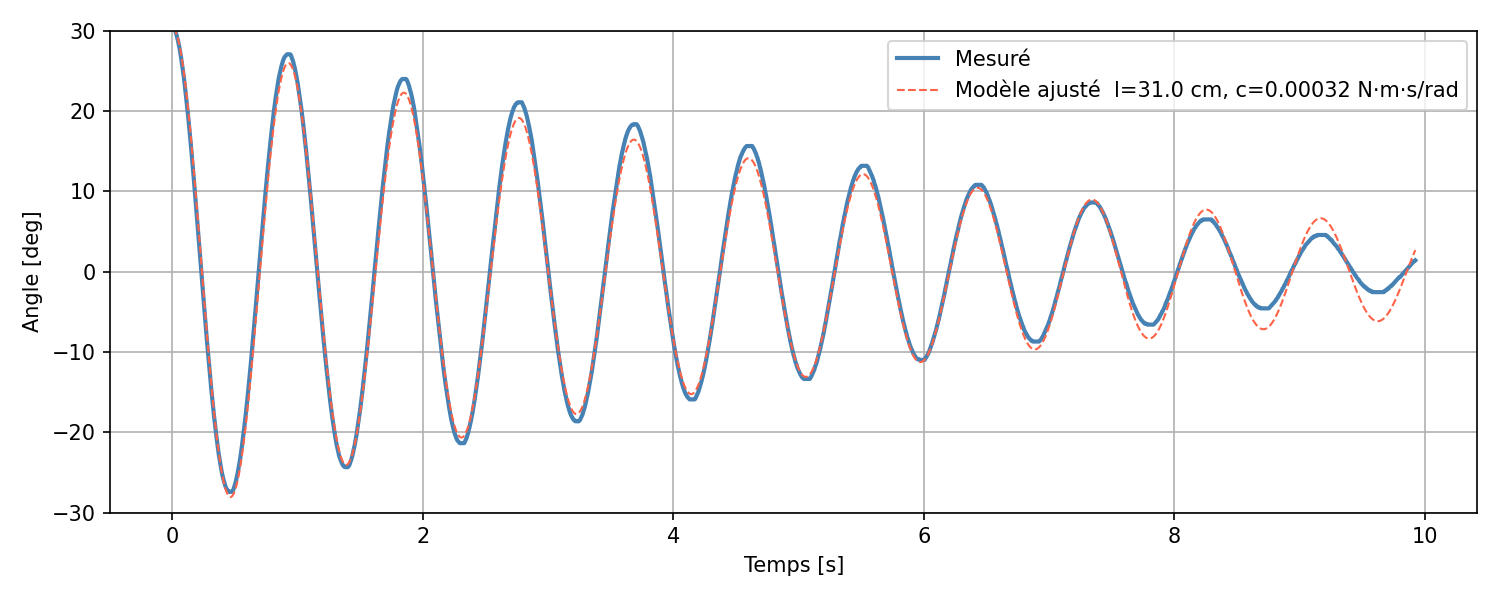
\includegraphics[width=\linewidth]{figures/free_response_fit.png}
\end{figure}

\end{frame}


% La 3e partie: Controle par PID
% Le titre de la partie
\section{Stabilisation de la dynamique par contrôle PD}

%%%%%%%%%%%%%%%%%%%%%%%%%%%%%%%%%%%%%%%%%%%%%%%%

\begin{frame}
\frametitle{Contrôle PD}
\framesubtitle{Schéma block du contrôle du pendule inversé}

\begin{center}
\begin{tikzpicture}[>=Stealth, auto,
    block/.style={draw, rectangle, rounded corners=3pt, fill=blue!8,
                  minimum height=1.0cm, minimum width=2.2cm,
                  align=center, font=\small},
    sum/.style  ={draw, circle, minimum size=0.65cm, inner sep=0pt},
    node distance=0pt
  ]

  % Nodes
  \node[sum] (sum) {};
  \node[block, right=1.2cm of sum] (pd)    {Contrôleur\\PD};
  \node[block, right=1.8cm of pd]  (plant) {Pendule\\inversé};

  % Summing junction +/-
  \node[font=\footnotesize, below left=2pt and 2pt of sum] {$-$};

  % Input: theta_ref
  \draw[->] (sum.west) ++(-1.5,0) node[above right] {$\theta_\mathrm{ref} = \pi$} -- (sum.west);

  % sum -> PD
    \draw[->] (sum.east) -- node[midway, above] {$\varepsilon_\theta(t)$} (pd.west);

  % PD -> plant
    \draw[->] (pd.east) -- node[midway, above] {$u(t) = \ddot{x}(t)$} (plant.west);

  % plant -> output
    \draw[->] (plant.east) node[above right] {$\theta(t)$} -| ++(1.0, -1.0) -| (sum.south);
\end{tikzpicture}
\end{center}

\vspace{0.3cm}

\[
  u(t) = \underbrace{k_p \cdot \varepsilon_\theta(t)}_{\text{Proportionnel}}
        + \underbrace{k_d \cdot \frac{\mathrm{d} \varepsilon_\theta(t)}{\mathrm{d} t}}_{\text{Dérivé}}
\]

\end{frame}

%%%%%%%%%%%%%%%%%%%%%%%%%%%%%%%%%%%%%%%%%%%%%%%%

\begin{frame}
\frametitle{Contrôle PD}
\framesubtitle{Contrôleur Proportionnel}

Avec $u = -k_p\,\varphi$, l'équation linéarisée devient :
\[
  D\,\ddot{\varphi} + c\,\dot{\varphi} + (ml\,k_p - mgl)\,\varphi = 0
\]
Stabilité (Routh-Hurwitz~\cite{routh_hurwitz}) $\Rightarrow$ $ml\,k_p > mgl$, soit :
\[
  k_{p,c} = g + \frac{c^2}{4mlD} \approx g \approx 9{,}81 \ \mathrm{m/s^2}
\]

% \vspace{0.2cm}

\begin{columns}[T]
  \begin{column}{0.48\textwidth}
    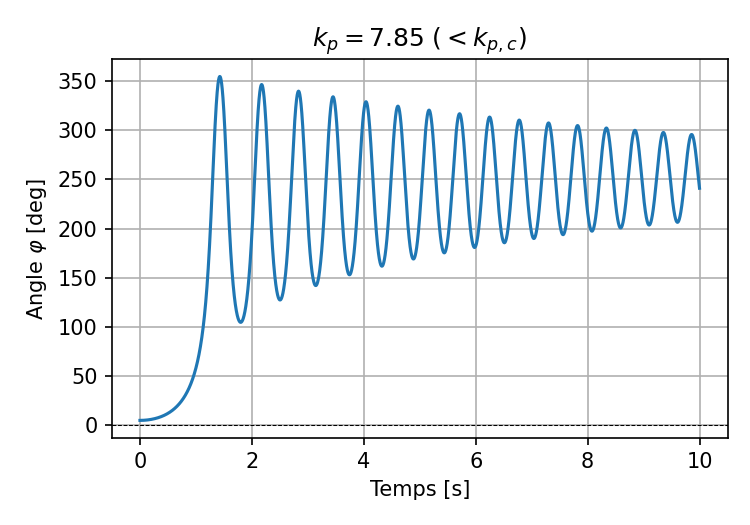
\includegraphics[width=\linewidth]{figures/kp_below.png}
  \end{column}
  \begin{column}{0.48\textwidth}
    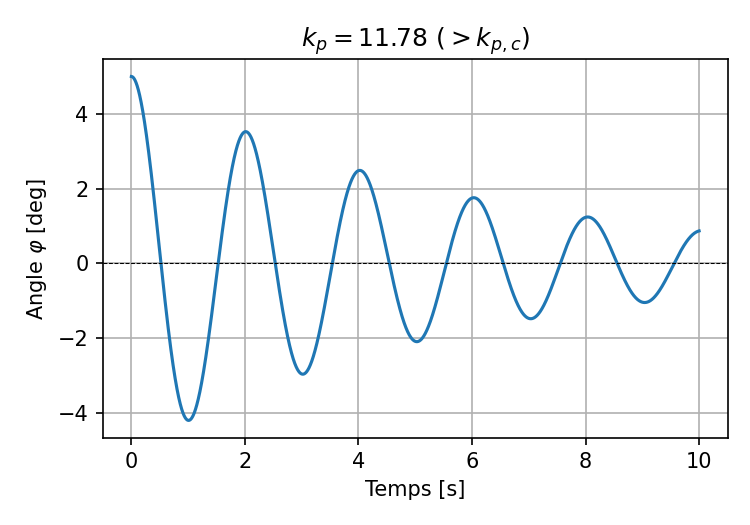
\includegraphics[width=\linewidth]{figures/kp_above.png}
  \end{column}
\end{columns}

\end{frame}

%%%%%%%%%%%%%%%%%%%%%%%%%%%%%%%%%%%%%%%%%%%%%%%%

\begin{frame}
\frametitle{Contrôle PD}
\framesubtitle{Contrôleur Dérivatif}

% Expliquer comment le contrôleur derivatif modifie la dynamique du système: ça ajoute de l'amortissement.
% Ca peut être important pour le confort sur un segway par exemple.

Avec $u = -k_p\,\varphi - k_d\,\dot{\varphi}$, l'équation linéarisée devient :
\[
  D\,\ddot{\varphi} + (c + ml\,k_d)\,\dot{\varphi} + (ml\,k_p - mgl)\,\varphi = 0
\]
Amortissement critique:
\[
  k_{d,c} = \frac{1}{ml}\!\left(2\sqrt{D\,(ml\,k_p - mgl)} - c\right)
\]

\begin{figure}
    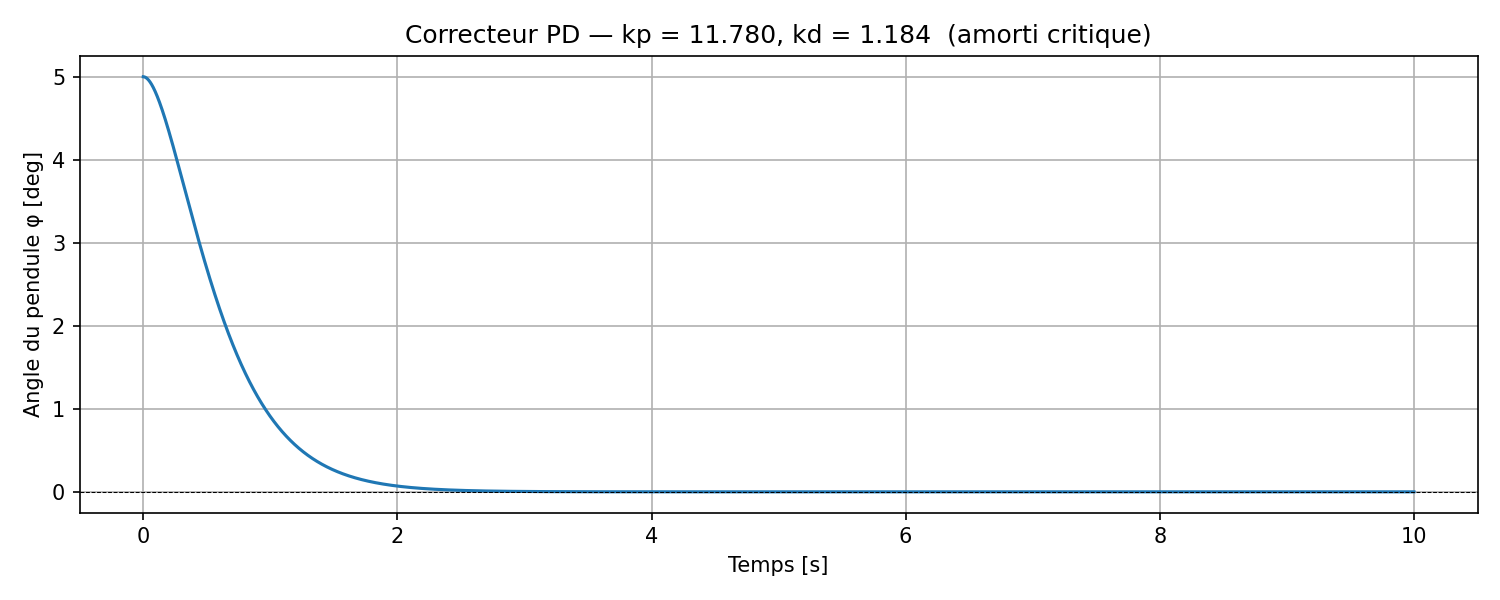
\includegraphics[width=0.8\linewidth]{figures/kp_kd.png}
\end{figure}

\end{frame}

%%%%%%%%%%%%%%%%%%%%%%%%%%%%%%%%%%%%%%%%%%%%%%%%

\begin{frame}
\frametitle{Contrôle PD}
\framesubtitle{Résultats expérimentaux}

\begin{figure}
    \only<1>{%
        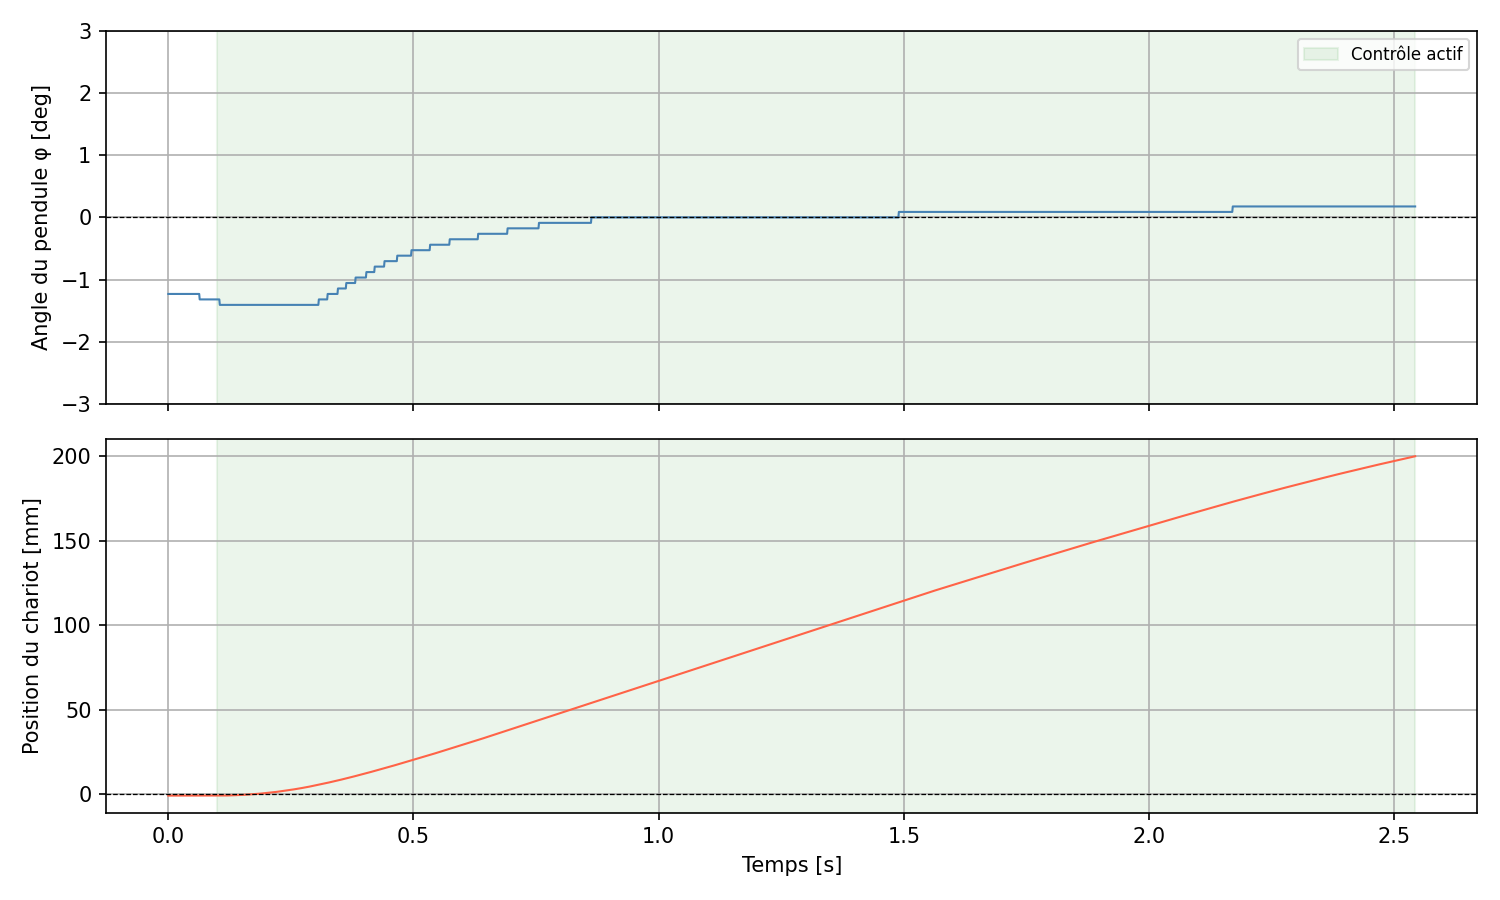
\includegraphics[width=0.85\linewidth]{figures/kp_12_kd_1_stable_bis.png}\\[2pt]
        {\scriptsize Résultats expérimentaux — $k_p = 12$, $k_d = 1$}
    }%
    \only<2>{%
        Même comportement en simulation:
        $\phi$ est correctement stabilisé, mais le chariot n'est pas stable.

        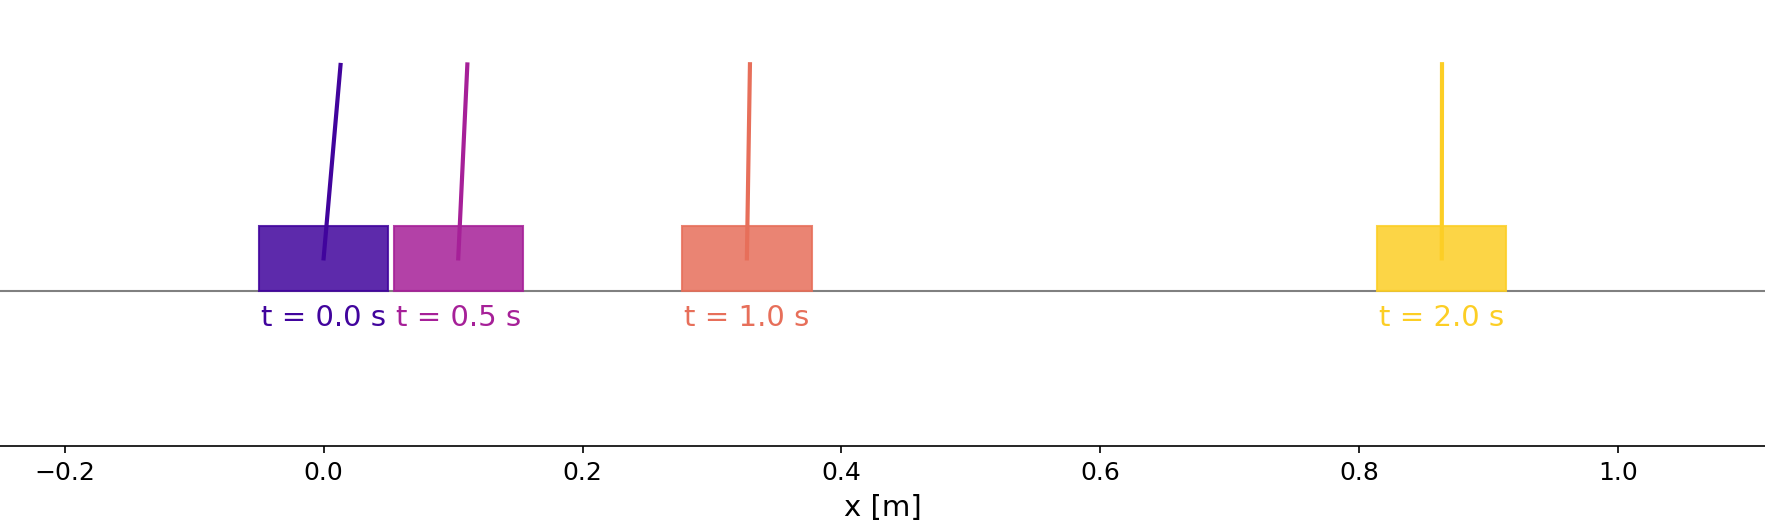
\includegraphics[width=\linewidth]{figures/snapshots_simulation_kp_kd_1.png}\\[2pt]
        {\scriptsize Résultats de simulation — $k_p = 12$, $k_d$}

        \vspace{1em}

        Pour contrôler à la fois $\phi$ et $x$, le contrôleur PD n'est pas adapté.
    }
\end{figure}

\end{frame}




% La 4e partie: Controle par LQR
\section{Stabilisation de la dynamique par contrôle LQ}

%%%%%%%%%%%%%%%%%%%%%%%%%%%%%%%%%%%%%%%%%%%%%%%%

\begin{frame}
\frametitle{Contrôle LQ}
\framesubtitle{Modèle d'état — Commande par retour d'état}

Modèle par représentation d'états:
\[
    \mathbf{X} =
    \begin{pmatrix} x \\ \dot{x} \\ \varphi \\ \dot{\varphi} \end{pmatrix}, \quad
        \dot{\mathbf{X}} = A\mathbf{X} + B u, \quad
        A = \begin{pmatrix}
            0 & 1 & 0 & 0 \\
            0 & 0 & 0 & 0 \\
            0 & 0 & 0 & 1 \\
            0 & 0 & \tfrac{mgl}{D} & -\tfrac{c}{D}
        \end{pmatrix}, \quad
        B = \begin{pmatrix} 0 \\ 1 \\ 0 \\ \tfrac{ml}{D} \end{pmatrix}
        \]

\vspace{1em}

Commande par retour d'état:

\vspace{1em}

\begin{tikzpicture}[>=Stealth, auto,
    block/.style={draw, rectangle, rounded corners=3pt, fill=blue!8,
                  minimum height=0.9cm, minimum width=2.0cm,
                  align=center, font=\small},
    sum/.style={draw, circle, minimum size=0.6cm, inner sep=0pt},
    node distance=0pt
  ]
  \node[sum] (sum) {};
  \node[font=\footnotesize, below left=0pt of sum] {$-$};
  \node[block, right=1.0cm of sum] (K) {$\mathbf{K}$};
  \node[block, right=1.0cm of K]   (plant) {Pendule\\inversé};

  % X_ref input
  \draw[->] (sum.west) ++(-1.2,0) node[above right] {$\mathbf{X}_\mathrm{ref}$} -- (sum.west);

  % sum -> K
  \draw[->] (sum.east) -- (K.west);

  % K -> plant
  \draw[->] (K.east) -- node[midway, above] {$u(t)$} (plant.west);

  % plant output + feedback
  \draw[->] (plant.east) node[above right] {$\mathbf{X}(t)$} -| ++(0.7,-1.0) -| (sum.south);
\end{tikzpicture}

\vspace{0.3cm}
\[
  u(t) = \mathbf{K}\,\bigl(\mathbf{X}_\mathrm{ref} - \mathbf{X}(t)\bigr), \quad
  \mathbf{K} = \begin{bmatrix} k_x & k_{\dot x} & k_\varphi & k_{\dot\varphi} \end{bmatrix}
\]

\end{frame}

%%%%%%%%%%%%%%%%%%%%%%%%%%%%%%%%%%%%%%%%%%%%%%%%

\begin{frame}
\frametitle{Contrôle LQ}
\framesubtitle{Choix de la matrice de retour d'état}

Explication de la synthèse (Riccati).
Minimisation quadratique de certains états.
Exemple de valeurs obtenues pour une synthèse.

\end{frame}

%%%%%%%%%%%%%%%%%%%%%%%%%%%%%%%%%%%%%%%%%%%%%%%%

\begin{frame}
\frametitle{Contrôle LQ}
\framesubtitle{Simulation}

\begin{columns}[T]
  \begin{column}{0.5\textwidth}
    \centering
    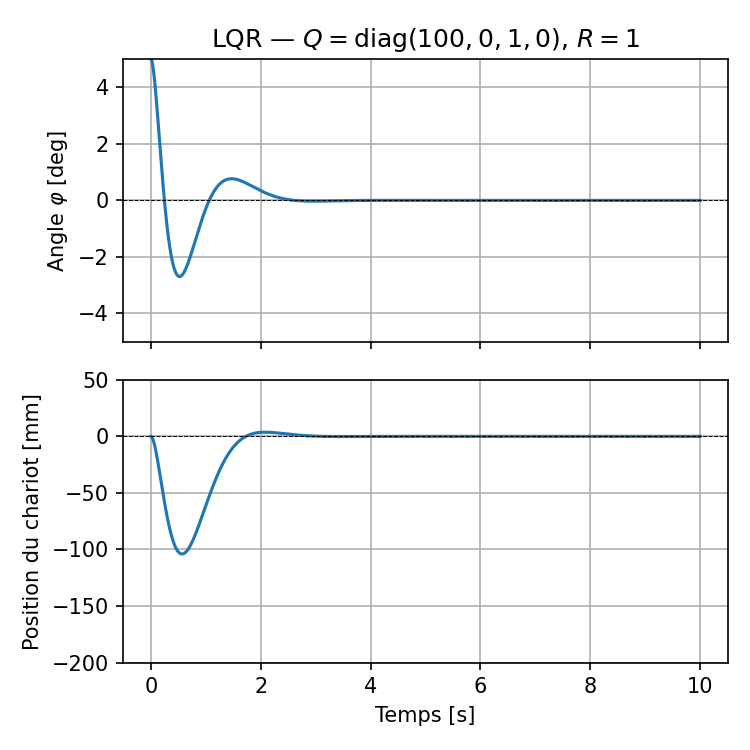
\includegraphics[width=\linewidth]{figures/lqr_x100_xd0_th1_thd0_u1.png}\\[2pt]
    {\scriptsize Pondération forte sur $x$: $q_x = 100$, $q_\varphi = 1$}
  \end{column}
  \begin{column}{0.5\textwidth}
    \centering
    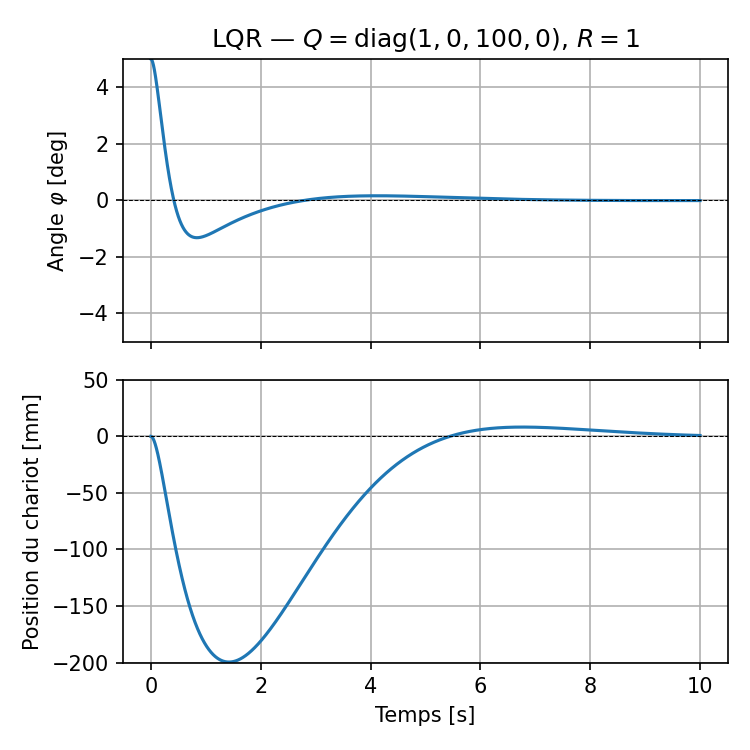
\includegraphics[width=\linewidth]{figures/lqr_x1_xd0_th100_thd0_u1.png}\\[2pt]
    {\scriptsize Pondération forte sur $\varphi$: $q_x = 1$, $q_\varphi = 100$}
  \end{column}
\end{columns}

\end{frame}

%%%%%%%%%%%%%%%%%%%%%%%%%%%%%%%%%%%%%%%%%%%%%%%%

\begin{frame}
\frametitle{Contrôle LQ}
\framesubtitle{Résultats Expérimentaux}

\begin{figure}
    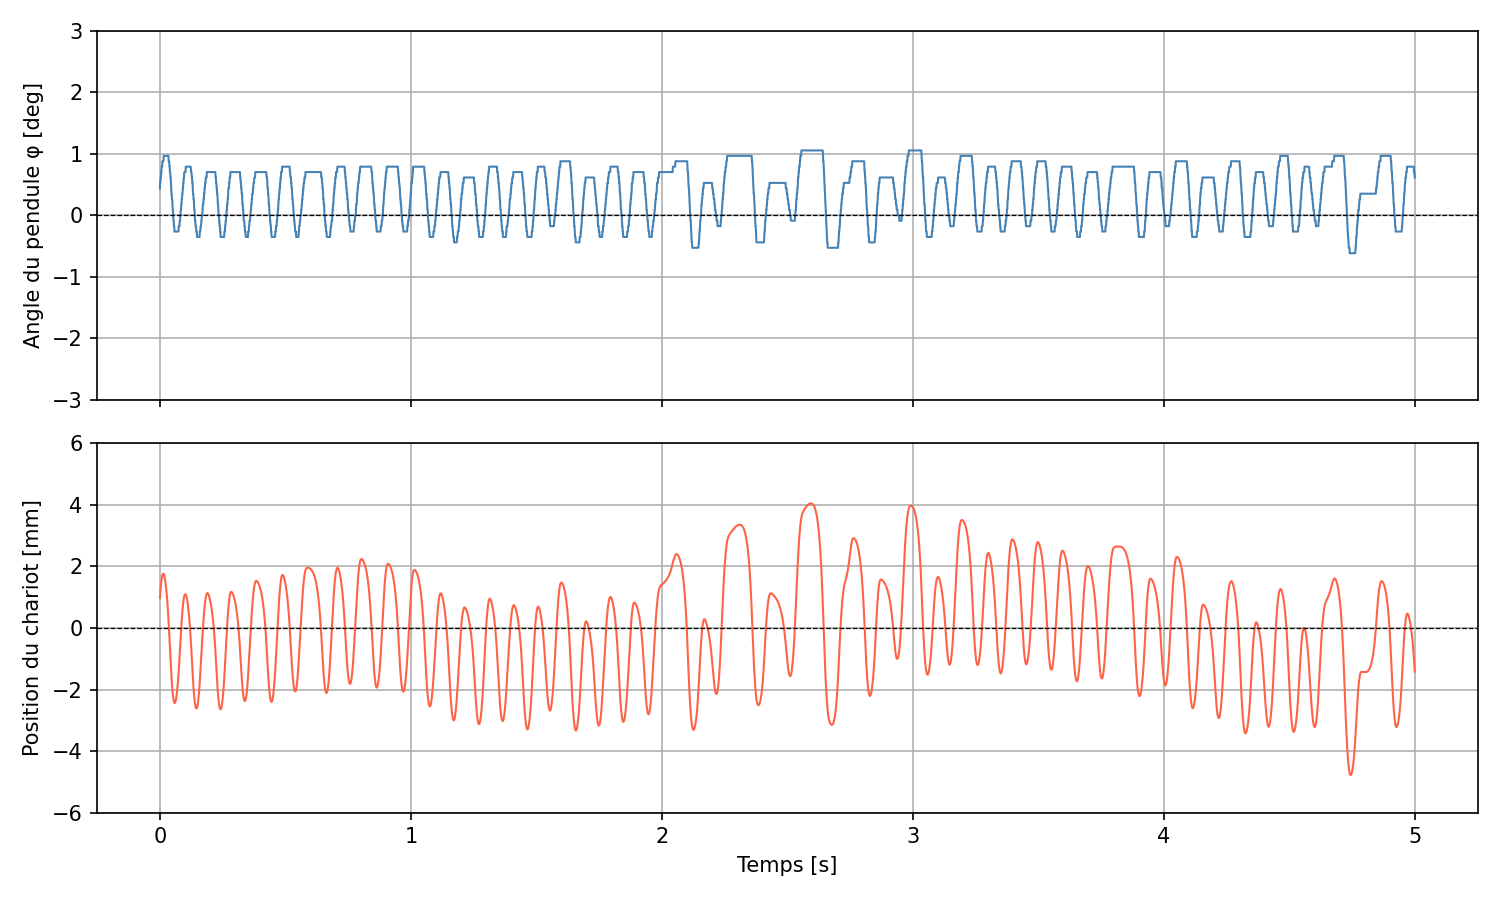
\includegraphics[width=0.9\linewidth]{figures/data_lqr_x1000_xd0_th_1000_thd0_u1_stability.png}\\[2pt]
    
    {\scriptsize $\mathbf{K} = [-31.6\ -23.1\ 92.8\ 18.3]$, stabilité observée de $\pm 1\,\text{deg}$, $\pm 5\,mm$}
\end{figure}

\end{frame}


% Conclusion
% Le titre de la partie
\section{Conclusion}

%%%%%%%%%%%%%%%%%%%%%%%%%%%%%%%%%%%%%%%%%%%%%%%%
% Première diapo avec un exemple de tableau
%%%%%%%%%%%%%%%%%%%%%%%%%%%%%%%%%%%%%%%%%%%%%%%%
\begin{frame}
\frametitle{Conclusion}

Conclusion du TIPE.

Ouverture? LQG? Explication différences modèle / expérience ? ...

\end{frame}

\begin{frame}[allowframebreaks]{Références}
  \printbibliography
\end{frame}

\end{document}


